\documentclass[10pt, twoside]{article}

\usepackage{float}
\usepackage{graphicx}

\begin{document}

%%%%%%%%%%%%%%%%%%%%%%%%%%%%%%%%%%%%%%%%%%%%%
% Project Description : 
%    Background information, goal for project
% No technical details. Explain to someone
% who has never heard of this project and 
% does not know about any particulars.
%%%%%%%%%%%%%%%%%%%%%%%%%%%%%%%%%%%%%%%%%%%%%
\section{Project Description}
The Amazing Race is a popular reality TV show currently in its $27^{th}$ season on
CBS where contestants compete in physical and mental challenges while travelling
around the world. Teams compete in stages. Each stage typically consists of two
rounds of challenges. In each round, teams typically get to choose to compete in
one of two challenges. Teams can switch challenges at any time during a stage.
The team that is last to complete the final challenge (or ‘check in’) in a stage
is usually disqualified. The remaining teams then begin the next stage in their
finishing order. This continues until there are three (or sometimes four) teams
left. A final challenge is then issued, and the winner of that challenge is the
winner of The Amazing Race. Winners at each individual stage receive a prize
(typically monetary or travel based), while the overall winners receive \$1,000,000.

There are also tactical maneuvers available to contestants. For example, a `Fast
Pass’, which lets a team skip a challenge, is occasionally offered to a single stage
winner. Also, `U-turns’ allow teams to force an opposing team to complete both
challenges at a single round of a single stage.

We propose building a computer system to analyze the early episodes of a
single season of The Amazing Race and predict the winning team. We think this
is a viable goal due to a few assumptions. First, the producers of the show need
to foster a relationship between the audience and the teams that are going to be
competing for a long time (i.e. the winners). Yes, each show must show a number
of teams to some extent - teams that fight, teams that win the stage, etc - but deep
storylines will only be developed for teams that last deep into the competition.
So, if an early episode has special interviews and extended scenes with a middling,
somewhat unremarkable team early in the season, that team probably goes a long
way. Also, a team that comes in second to last on Day 1 has a long, arduous
climb back into contention due to starting later than other teams in the next
stage. Performance within the actual race, therefore, seems to be another viable
predictor of the eventual winner. We believe a combination of these factors can be
leveraged to predict teams that last deep into the competition early in the season.

There is no real motivation for this project beyond personal skill development
(and enjoyment) through exploring and excercising with techniques in image
analysis and machine learning.

%%%%%%%%%%%%%%%%%%%%%%%%%%%%%%%%%%%%%%%%%%%%%
% Currently Available Solutions:
%     Self Explanatory
%%%%%%%%%%%%%%%%%%%%%%%%%%%%%%%%%%%%%%%%%%%%%
\subsection{Currently Available Solutions}
While there are a number of libraries and packages available for general prediction,
there is no database known to us that has the type of features of The Amazing
Race that would be useful for predicting the winner. Therefore, most of the
original contribution of this work comes from the construction of the feature vectors
themselves.

%%%%%%%%%%%%%%%%%%%%%%%%%%%%%%%%%%%%%%%%%%%%%
% Module Design:
%     High level technical details, flow of
% information and steps taken to run/use any
% product.
%%%%%%%%%%%%%%%%%%%%%%%%%%%%%%%%%%%%%%%%%%%%%
\section{Module Design}
There will be two main systems in the project. The first system extract data from
The Amazing Race episodes in a format while the second system uses that data
to calculate win probabilities for each competing team. The first system consists
of two modules : a feature extraction module (FEM) that takes screenshots of
The Amazing Race episodes, identifies attributes for each team, and constructs
the feature vectors, and a feature validation module (FVM) which constructs a
user-defined mapping from screenshots to teams and validates team identification
in the FEM. The second system is a single module, which consists of a prediction
algorithm, taking feature vectors from the FEM and calculating win probabilities.

\subsection{Technologies Used}
Our system will be developed exclusively in MATLAB, using ffmpeg to extract
screenshots from episodes.

\subsection{Feature Extraction System}
The feature extraction system is responsible for formatting episodes of The Amazing Race into
data suitable to predict from. The extraction is done by first automatically
detecting the prominence of each team in each episode, mapping episode portions
to teams. Stats are then calculated and combined into feature vectors. In order
to make sure the mapping from teams to episode portions is reasonable, a second
process is available that uses user input to construct a ground truth mapping on
a subset of episode data which can be used for comparison. Figure \ref{fig:feature_extraction_module}
shows a high level description of the workflow.

\label{section:FES}
\begin{figure}[H]
  \centering
  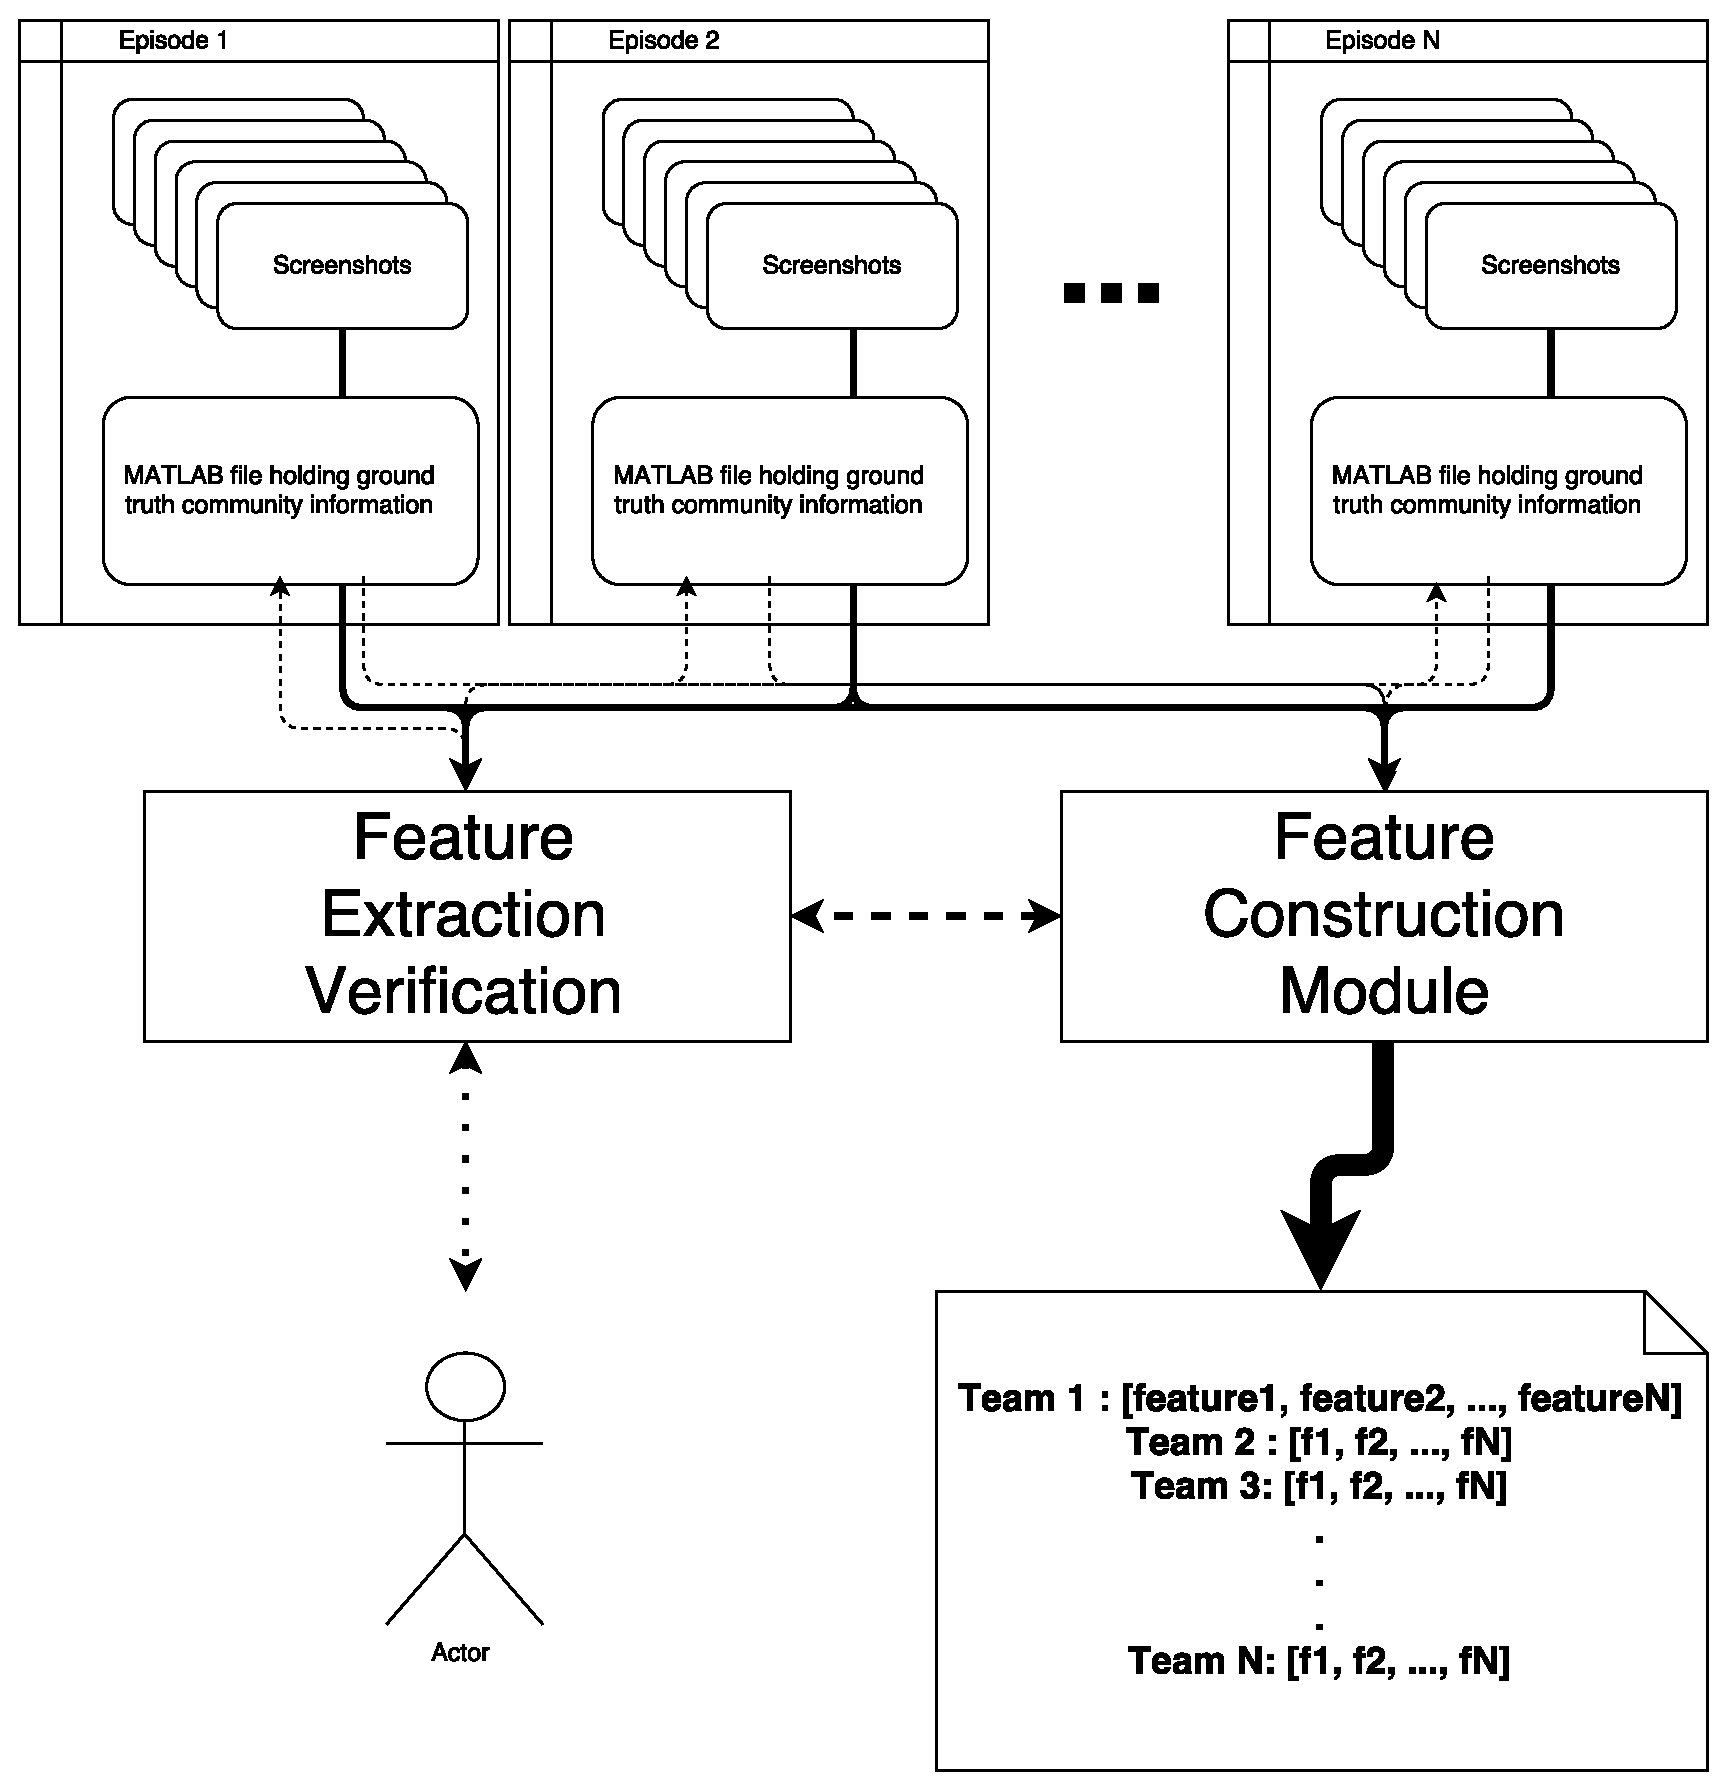
\includegraphics[width=\textwidth]{FeatureExtractionModule}
  \caption{The Amazing Race Feature Extraction Module}
  \label{fig:feature_extraction_module}
\end{figure}

Figure \ref{fig:feature_extraction_module_details} shows a more detailed version of the workflow.

\begin{figure}[H]
  \centering
  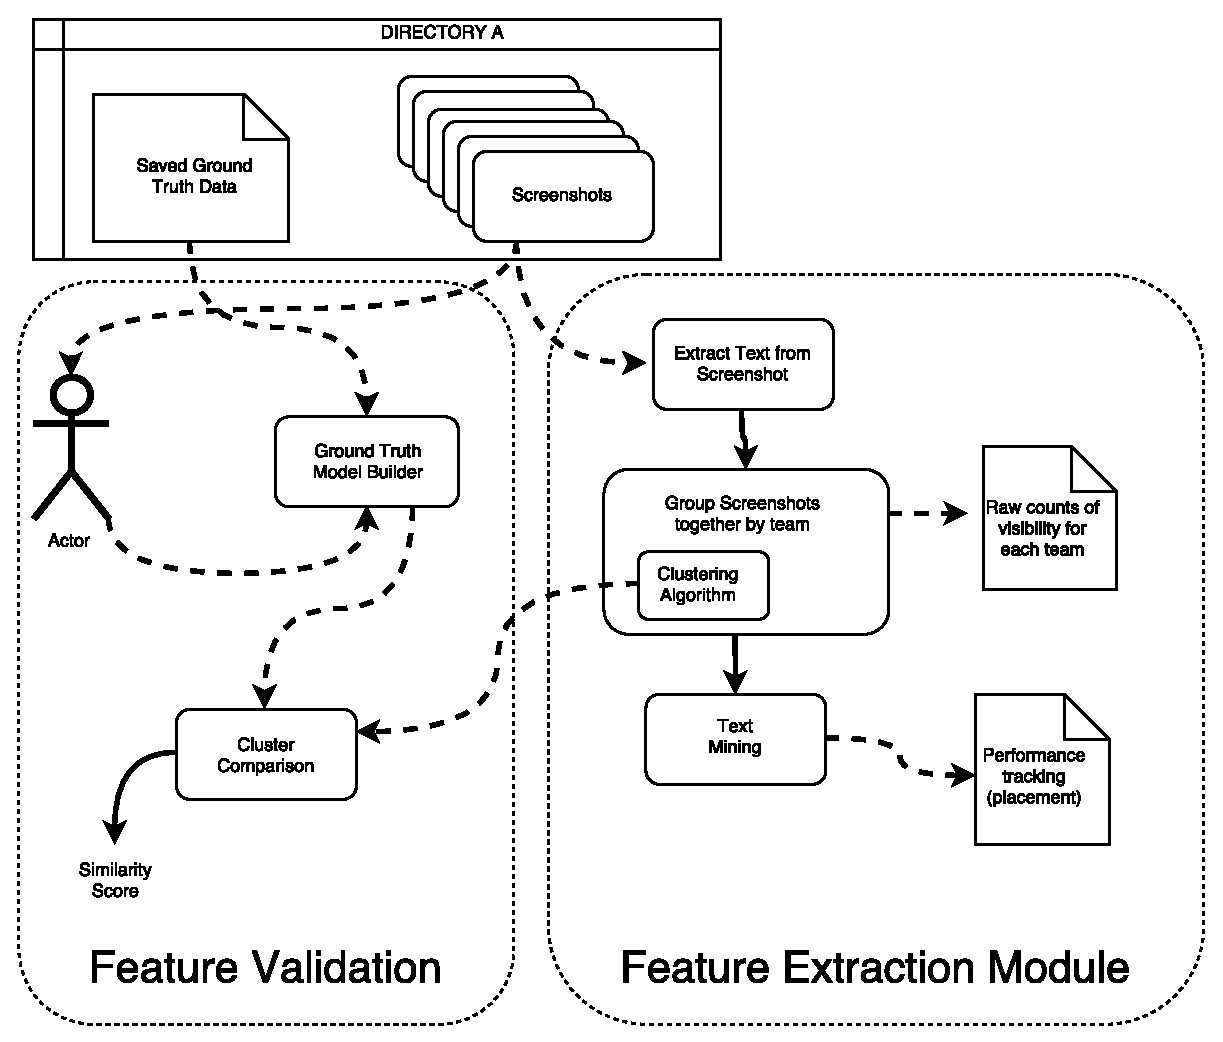
\includegraphics[width=\textwidth]{ExtractionDetails}
  \caption{A More Detailed Look At The Amazing Race Feature Extraction Module}
  \label{fig:feature_extraction_module_details}
\end{figure}

\subsection{Prediction System}
\label{section:PS}
Currently basically undesigned. See Fig.~\ref{fig:prediction_module} for an 
extremely simple first pass.

The prediction system is a straight forward application of some prediction algorithm
on the feature vector. By design, the system outputs probabilities that each
team will win. The system may also output an (unweighted) order of teams, in
decreasing likelihood of winning (basically declaring the finishing order).

\begin{figure}[H]
  \centering
  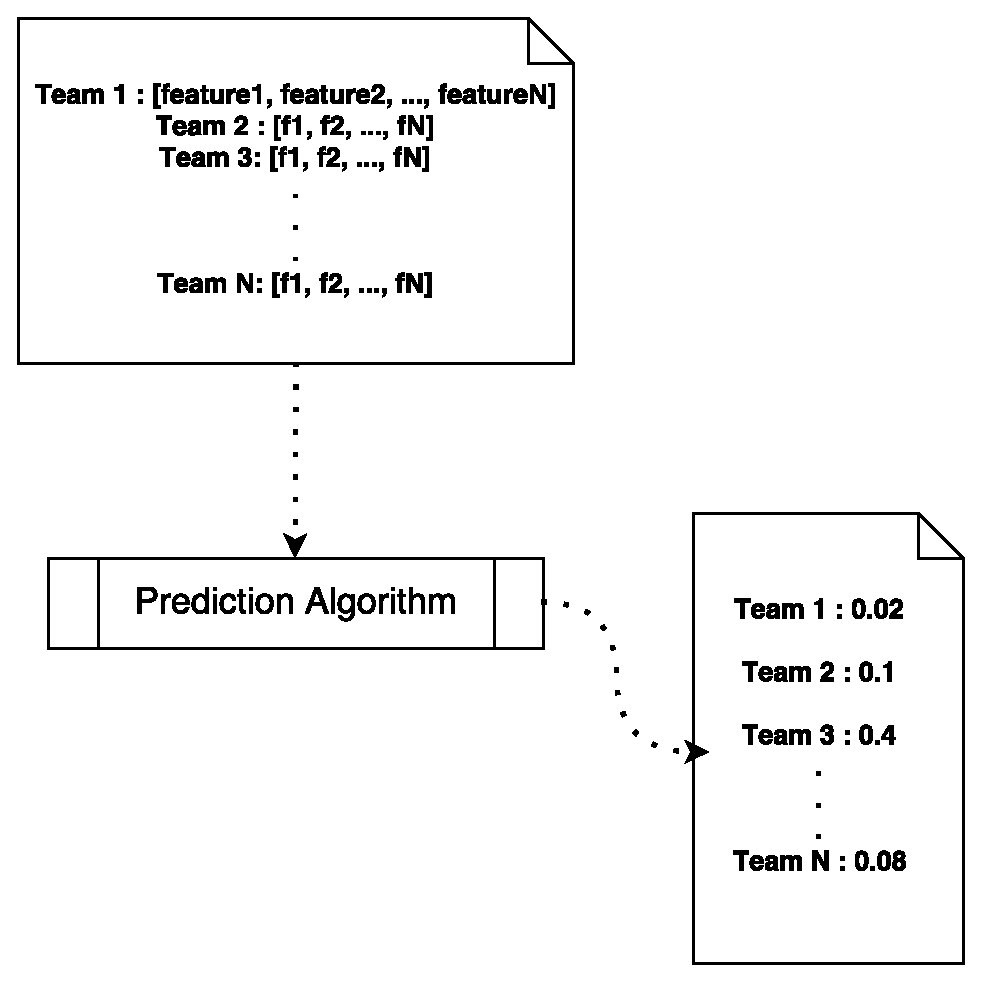
\includegraphics[width=\textwidth]{PredictionModule}
  \caption{Validation Module Flow}
  \label{fig:prediction_module}
\end{figure}

%%%%%%%%%%%%%%%%%%%%%%%%%%%%%%%%%%%%%%%%%%%%%
% Code Design: 
%     Low level description - specific
% functions and coupling between segments.
%%%%%%%%%%%%%%%%%%%%%%%%%%%%%%%%%%%%%%%%%%%%%
\section{Code Design}

The following is a list of the code found in each specific file in the project.
Figure \ref{fig:class_diagram_validate} shows the coupling between files. For more information,
see the comments in the files.

%%%%%%%%%%%%%%%%%%%%%%%%%%%%%%%%%%%%%%%%%%%%
% Try to keep this sorted by filename
%%%%%%%%%%%%%%%%%%%%%%%%%%%%%%%%%%%%%%%%%%%%
  \paragraph{amazing\_race.m}
  \paragraph{amazing\_race\_segmenter.m}
  \paragraph{subimage\_distance.m}
  Holds functions for comparing two binary matrices of the same dimension.
  \paragraph{subset\_distance\_hierarchical.m}

\begin{figure}[H]
  \centering
  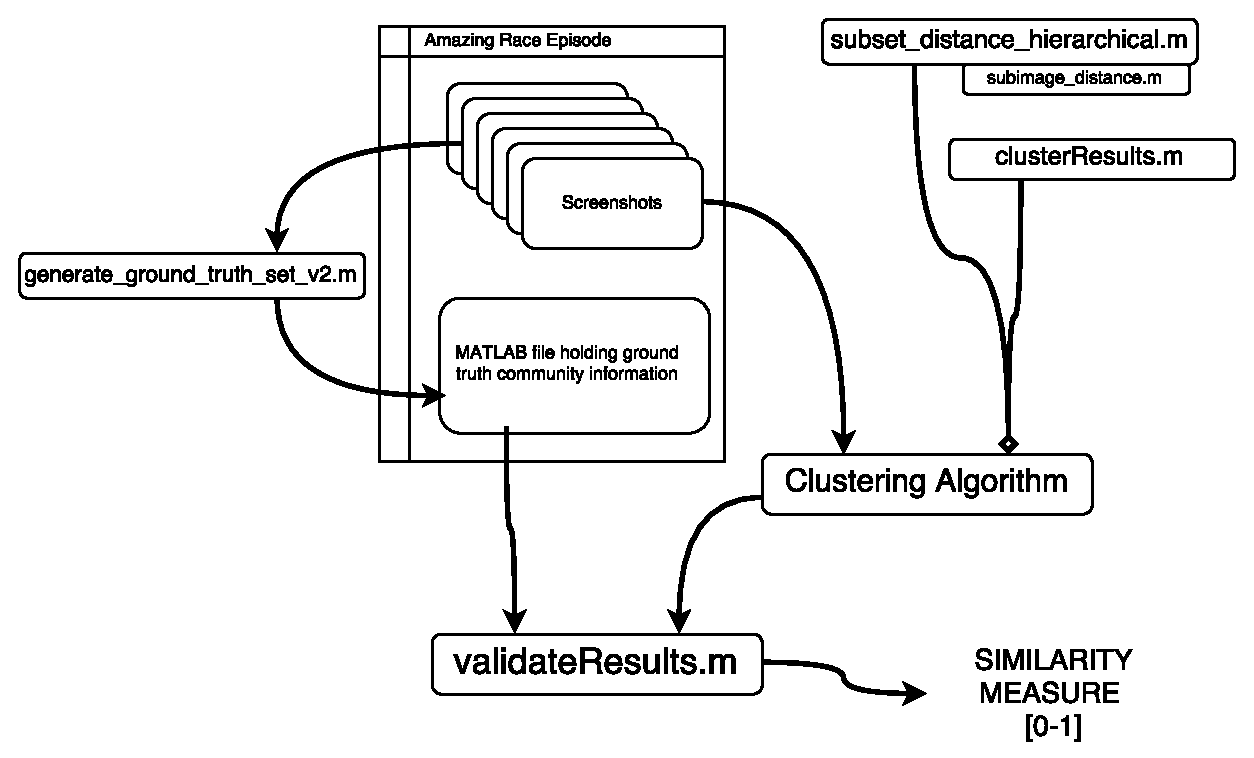
\includegraphics[width=\textwidth]{ClassDiagramValidate}
  \caption{Detailed Explanation of Validation Architecture}
  \label{fig:class_diagram_validate}
\end{figure}

%%%%%%%%%%%%%%%%%%%%%%%%%%%%%%%%%%%%%%%%%%%%%
% Document Information: 
%    Metadata, revision history, indices, 
% glossary, etc.
%%%%%%%%%%%%%%%%%%%%%%%%%%%%%%%%%%%%%%%%%%%%%
\section{Document Information}

\subsection{Glossary}
\begin{itemize}
\item[] \textbf{FEM (Section ~\ref{section:FES})} : Feature Extraction Module
\item[] \textbf{FVM (Section ~\ref{section:FES})} : Feature Validation Module
\item[] \textbf{PM (Section ~\ref{section:PS})} : Prediction Module
\end{itemize}

\subsection{Document History}
\begin{tabular}{|p{0.15\textwidth}|p{0.25\textwidth}|p{0.5\textwidth}|p{0.1\textwidth}|} \hline
Date & Authors & Notes & Version \\ \hline
2015-10-22 & James Thompson & Recovered information (lost
due to github commit error) & 0.0.2 \\ \hline
\end{tabular}

\subsection{References}
Charts were developed using draw.io online tool.

\end{document}
